\chapter{Horizons de Sitter et probabilité cosmologique}

\lectureoverview{Un horizon n’est pas simplement une frontière causale. Pour un observateur stationnaire, c’est un système thermique : un thermomètre maintenu à une distance propre \(\rho\) de l’horizon indique une température de l’ordre de \(1/(2\pi\rho)\), tandis que le décalage gravitationnel vers le rouge rend le rayonnement observé de loin beaucoup plus froid. Nous transposerons cette leçon des trous noirs à l’espace de de Sitter, déduirons le rayon d’horizon constant \(H^{-1}\) et écrirons la métrique de la région statique de l’observateur. La seconde moitié du cours suit les conséquences troublantes de cette thermodynamique : entropie de de Sitter finie, récurrences de Poincaré, cerveaux de Boltzmann, inflation éternelle et problème de la mesure. Une dernière discussion distingue les structures supersymétriques exactes de la théorie des cordes du cadre encore inconnu qui pourrait décrire notre monde.}

\section{Ce que signifie la température d’un horizon}

Nous commençons avant le cours proprement dit par la question qui en déterminera l’orientation.

\begin{classroomqa}
\audiencequestion{Un horizon cosmique ne contient aucun trou noir. Par quel mécanisme peut-il néanmoins être chaud ?\lecturetimestamp{00:00:17}}
\lecturerresponse{Le mécanisme est le même que pour un horizon de trou noir. La question utile est opérationnelle : qu’indique un thermomètre maintenu près de l’horizon, et quel rayonnement parvient à un observateur qui en est éloigné ?}
\end{classroomqa}

La première expérience est locale. Maintenons un thermomètre à distance propre \(\rho\) de n’importe quel horizon régulier non extrémal. Assez près de l’horizon, la géométrie prend la forme universelle de Rindler, et le thermomètre indique
\begin{equation}
T_{\rm local}(\rho)\simeq \frac{1}{2\pi\rho}
\label{eq:l09-local-temperature}
\end{equation}
avec les unités où \(\hbar=c=k_B=1\). En rétablissant les constantes, on obtient
\begin{equation}
k_B T_{\rm local}(\rho)\simeq \frac{\hbar c}{2\pi\rho}.
\end{equation}
La divergence lorsque \(\rho\to0\) ne signifie pas qu’un observateur en chute libre rencontre une fournaise matérielle ordinaire. C’est la température attribuée par un observateur qui reste stationnaire juste à l’extérieur de l’horizon et doit donc accélérer de plus en plus violemment.

La conversation d’ouverture distingue aussi trois notions que l’on confond facilement : l’énergie, la température et l’entropie.

\begin{classroomqa}
\audiencequestion{Si des photons sont envoyés dans un trou noir, mesure-t-on toujours la même entropie, ou seule l’énergie change-t-elle ?\lecturetimestamp{00:01:22}}
\lecturerresponse{Dès qu’un photon devient inaccessible derrière l’horizon, une information supplémentaire est cachée. Dans le langage simplifié des bits employé ici, un photon peut cacher un bit supplémentaire et ainsi augmenter l’entropie. L’énergie, la température et l’entropie sont liées, mais elles ne sont pas interchangeables.}
\end{classroomqa}

\editorialnote{Pour un trou noir physique, la variation d’entropie est déterminée thermodynamiquement par \(dS=dE/T_H\) ; elle ne vaut pas universellement un bit pour chaque photon, quelle que soit son énergie. L’énoncé d’un bit est une idéalisation de la théorie de l’information utilisée dans le cours.}

La région proche de l’horizon émet et réabsorbe continuellement des fluctuations quantiques de haute fréquence. Pour l’observateur stationnaire, l’horizon rend ces fluctuations thermiques. Cela soulève pourtant immédiatement une énigme. Si la région est arbitrairement chaude, pourquoi un observateur éloigné n’est-il pas aveuglé par des photons d’énergie arbitrairement élevée ?

\section{Décalage vers le rouge et température de Hawking}

Une paroi chaude ordinaire reste une source de rayonnement de haute fréquence même lorsqu’on s’en éloigne. L’horizon est différent, car son rayonnement doit remonter le gradient de potentiel gravitationnel et subir un décalage vers le rouge. La vitesse du photon reste \(c\) ; c’est son énergie qui diminue,
\begin{equation}
E=\hbar\omega,
\qquad
\omega_{\rm received}<\omega_{\rm emitted}.
\end{equation}
L’analogie avec le morceau de craie, utilisée dans le cours, n’est valable que jusque-là. Une pierre lancée ralentit en s’élevant, tandis qu’un photon continue à la vitesse de la lumière, même si sa fréquence et son énergie diminuent.

Pour un trou noir de Schwarzschild, la température mesurée par un observateur à l’infini est
\begin{equation}
T_H=\frac{1}{8\pi M}
\label{eq:l09-hawking-natural}
\end{equation}
avec les unités \(G_N=\hbar=c=k_B=1\). En unités usuelles,
\begin{equation}
T_H=\frac{\hbar c^3}{8\pi G_N M k_B}.
\label{eq:l09-hawking-full}
\end{equation}

\begin{figure}[htbp]
\centering
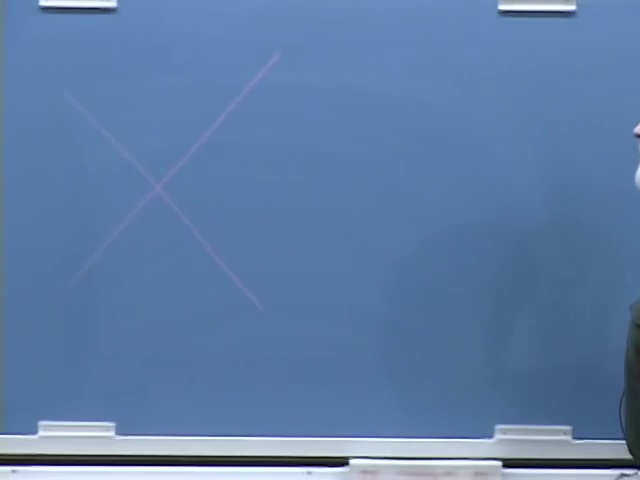
\includegraphics[width=0.68\textwidth]{lecture_09_figure_02.png}
\caption{La température de Hawking \(T_H=1/(8\pi M)\) en unités naturelles.}
\lectureframe{00:08:12}
\end{figure}

Un trou noir plus massif est plus froid. Le cours l’explique en retraçant le parcours d’un photon typique à rebours. Les photons thermiques ont une énergie caractéristique \(E_\gamma\sim T_H\). Un photon qui atteint l’infini avec une énergie de l’ordre de \(M^{-1}\) avait une énergie locale bien plus grande près de l’horizon, là où il a été émis. Le décalage vers le rouge entre la couche proche de l’horizon et l’infini est plus prononcé pour un trou noir plus massif, d’où une température asymptotique plus basse.

\begin{classroomqa}
\audiencequestion{Si le temps de Schwarzschild se fige à l’horizon, faut-il suivre le photon qui est tombé au départ et a formé le trou noir ?\lecturetimestamp{00:04:19}}
\lecturerresponse{Pour répondre à la question de la température, suivons les photons émis vers l’extérieur. Ils partent à une fréquence locale très élevée, perdent de l’énergie en remontant et arrivent sous forme de rayonnement de Hawking. Le devenir du photon initialement tombé est une question distincte, qui concerne l’information.}
\end{classroomqa}

\section{La couche de Planck et l’horizon étiré}

Jusqu’à quelle distance peut-on se fier à la relation locale de l’équation~\eqref{eq:l09-local-temperature} ? Dans le cours, la longueur de Planck est considérée comme la plus petite distance ayant un sens dans la description semi-classique. Cela suggère l’existence d’une mince couche, située à peu près à une longueur de Planck à l’extérieur de l’horizon mathématique, remplie de fluctuations à l’échelle de Planck. Elle émet et absorbe continuellement.

La plupart des quanta émis ne s’échappent pas. Seuls ceux qui sont dirigés dans un cône sortant très étroit évitent de retomber. Les quanta émis dans des directions génériques reviennent vers l’horizon. Les excitations sortantes et entrantes entrent en collision et produisent des paires ainsi que d’autres particules ; en ce sens, la description stationnaire comporte une fine coquille de matière extrêmement chaude.

\begin{figure}[htbp]
\centering
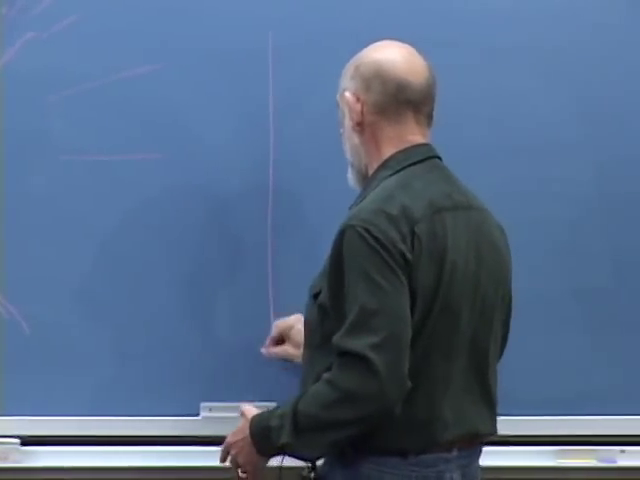
\includegraphics[width=0.74\textwidth]{lecture_09_figure_03.png}
\caption{Le cône d’échappement étroit du rayonnement proche de l’horizon. La plupart des quanta émis localement reviennent vers l’horizon.}
\lectureframe{00:11:38}
\end{figure}

Il existe une représentation complémentaire dans l’espace-temps. Loin d’un horizon, une fluctuation virtuelle peut être représentée schématiquement par une petite boucle fermée : une excitation particule-antiparticule apparaît puis disparaît avant de pouvoir devenir un état asymptotique. Près d’un horizon, une fluctuation peut chevaucher la frontière causale. Pour l’observateur extérieur, la partie située à l’extérieur ressemble à une particule émise par l’horizon puis réabsorbée. Une très petite fraction s’échappe et devient du rayonnement de Hawking.

\begin{classroomqa}
\audiencequestion{Dans le diagramme extérieur, une telle fluctuation s’étend-elle de \(t=-\infty\) à \(t=+\infty\) ?\lecturetimestamp{00:15:00}}
\lecturerresponse{L’horizon classique exact conduit à cette description d’apparence singulière. En pratique, nous le remplaçons par un horizon étiré, une surface de genre temps située à environ une longueur de Planck à l’extérieur. L’émission et la réabsorption ont alors lieu à des temps extérieurs finis.}
\end{classroomqa}

\begin{figure}[htbp]
\centering
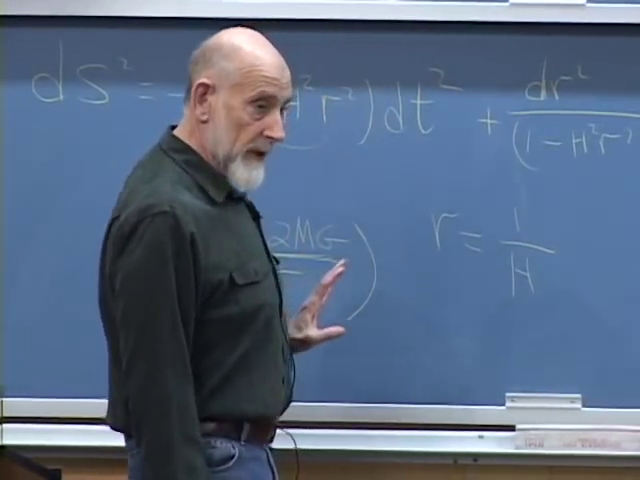
\includegraphics[width=0.72\textwidth]{lecture_09_figure_04.png}
\caption{L’horizon classique et l’horizon étiré voisin utilisé dans la description extérieure.}
\lectureframe{00:15:52}
\end{figure}

L’horizon étiré n’est pas une nouvelle frontière invariante. C’est une surface effective placée à l’endroit où la géométrie semi-classique cesse d’être fiable. Les fluctuations quantiques de la matière et de la géométrie elle-même brouillent la position exacte à l’échelle de Planck. Cette construction regroupe cette incertitude dans une surface où la description extérieure reste finie.

Rien dans cet argument local n’indique si l’horizon appartient à un trou noir ou à un univers en accélération. C’est le lien avec l’espace de de Sitter.

\section{L’espace de de Sitter en coordonnées en expansion}

Le cours proprement dit commence par le feuilletage spatialement plat de l’espace-temps de de Sitter,
\begin{equation}
ds^2=-dt^2+e^{2Ht}d\mathbf{x}^2,
\qquad
d\mathbf{x}^2=dx^2+dy^2+dz^2.
\label{eq:l09-flat-slicing}
\end{equation}
La constante \(H\) est le taux d’expansion de de Sitter. Le facteur apparaît sous la forme \(e^{2Ht}\) parce que la métrique mesure le carré des distances ; un intervalle de coordonnées fixe a pour longueur physique
\begin{equation}
D(t)=e^{Ht}\lvert\Delta\mathbf{x}\rvert.
\end{equation}

\begin{figure}[htbp]
\centering
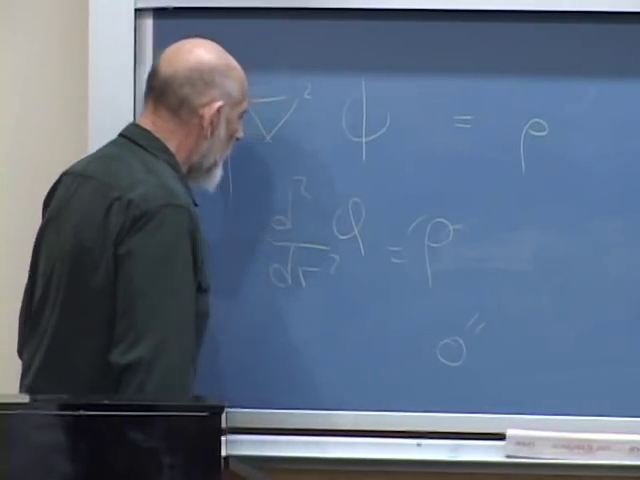
\includegraphics[width=0.78\textwidth]{lecture_09_figure_05.png}
\caption{La métrique de de Sitter en expansion exponentielle dans des coordonnées plates.}
\lectureframe{00:18:50}
\end{figure}

Ces coordonnées rendent l’expansion manifeste, mais placent l’infini futur à une distance infinie vers le haut de la page. Pour le faire apparaître au tableau, introduisons le temps conforme
\begin{equation}
\eta=-\frac{1}{H}e^{-Ht},
\qquad
-\infty<\eta<0.
\label{eq:l09-conformal-time}
\end{equation}
On a alors
\begin{equation}
dt=\frac{d\eta}{-H\eta},
\qquad
e^{Ht}=-\frac{1}{H\eta},
\end{equation}
et l’équation~\eqref{eq:l09-flat-slicing} devient
\begin{equation}
ds^2=\frac{1}{H^2\eta^2}
\left(-d\eta^2+d\mathbf{x}^2\right).
\label{eq:l09-conformal-metric}
\end{equation}
Lorsque \(t\to+\infty\), \(\eta\to0^{-}\). Un temps propre infini est ainsi comprimé sur la ligne horizontale finie \(\eta=0\).

\editorialnote{La transformation du temps est corrigée plusieurs fois pendant qu’elle est écrite au tableau. L’équation~\eqref{eq:l09-conformal-time} donne la forme cohérente : le début du temps cosmique correspond à \(\eta\to-\infty\) et l’infini futur à \(\eta\to0^{-}\).}

\begin{figure}[htbp]
\centering
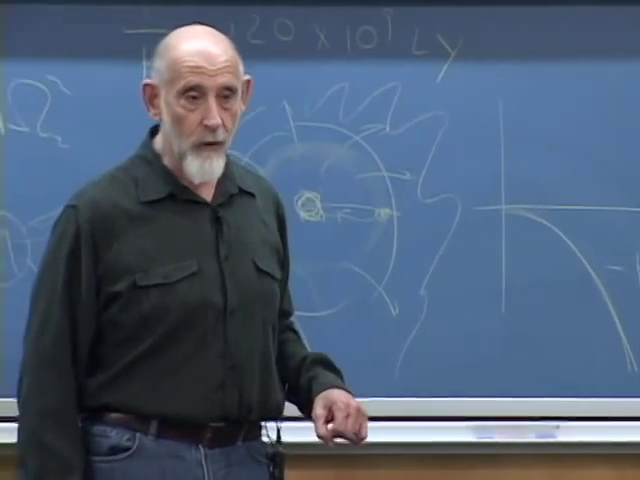
\includegraphics[width=0.82\textwidth]{lecture_09_figure_06.png}
\caption{La transformation vers le temps conforme et la métrique conformément plate.}
\lectureframe{00:21:24}
\end{figure}

Le facteur conforme multiplie les termes temporel et spatial ; il ne modifie donc pas les directions de genre nul. Pour un rayon lumineux radial,
\begin{equation}
ds^2=0
\quad\Longrightarrow\quad
-d\eta^2+dx^2=0
\quad\Longrightarrow\quad
\frac{dx}{d\eta}=\pm1.
\label{eq:l09-null-rays}
\end{equation}
La lumière se déplace donc à \(45^\circ\) dans le diagramme conforme. C’est ce qui rend ce changement de coordonnées utile : l’accessibilité causale devient visible.

\section{Le domaine causal d’un observateur}

Imaginons un observateur dont la ligne d’univers se prolonge pendant un temps propre infini. Sur le diagramme compactifié, elle aboutit en un point de \(\eta=0\). Tout signal que l’observateur peut recevoir se trouve dans le cône de lumière passé de ce point terminal. Les événements situés hors du cône ne peuvent jamais communiquer avec l’observateur, aussi longtemps qu’il attende.

\begin{figure}[htbp]
\centering
\includegraphics[width=0.78\textwidth]{lecture_09_figure_07.png}
\caption{Le cône de lumière passé limite d’un observateur dans les coordonnées conformes de de Sitter.}
\lectureframe{00:24:38}
\end{figure}

Un second observateur a un cône différent. Leurs domaines accessibles se recoupent, mais aucun des deux ne couvre tout l’espace-temps. Pour la suite de l’argument, adoptons le point de vue du premier observateur et appelons domaine causal de l’observateur ce cône de lumière passé.

Le dessin semble montrer que le domaine se rétrécit vers le futur, mais la largeur en coordonnées n’est pas une distance propre. Sur une tranche à temps constant \(\eta\), le carré de la distance physique entre l’observateur situé en \(x=0\) et l’horizon situé en \(x=\Delta x\) est
\begin{equation}
D^2=\frac{(\Delta x)^2}{H^2\eta^2}.
\label{eq:l09-horizon-distance-start}
\end{equation}
L’horizon est une droite de genre nul à \(45^\circ\) qui se termine en \(\eta=0\) ; par conséquent,
\begin{equation}
\Delta x=\lvert\eta\rvert.
\end{equation}
La substitution donne
\begin{equation}
D_{\rm hor}^2=\frac{1}{H^2},
\qquad
D_{\rm hor}=\frac{1}{H}.
\label{eq:l09-horizon-radius}
\end{equation}
La séparation en coordonnées diminue, mais le facteur conforme croît exactement de manière à compenser cette diminution. Le rayon propre de l’horizon est constant.

\begin{figure}[htbp]
\centering
\includegraphics[width=0.80\textwidth]{lecture_09_figure_08.png}
\caption{Dérivation au tableau qui transforme l’intervalle de coordonnées décroissant en la distance propre constante \(H^{-1}\).}
\lectureframe{00:28:42}
\end{figure}

\section{Le domaine statique}

Un rayon d’horizon constant suggère d’utiliser des coordonnées adaptées à l’observateur central. Sans dériver la transformation de coordonnées, le cours donne le résultat :
\begin{equation}
ds^2=
-\left(1-H^2r^2\right)d\tau^2
+\frac{dr^2}{1-H^2r^2}
+r^2d\Omega_2^2.
\label{eq:l09-static-patch}
\end{equation}
Les coefficients dépendent de \(r\), et non de \(\tau\). Cette carte couvre le domaine statique de l’observateur,
\begin{equation}
0\le r<\frac{1}{H}.
\end{equation}

\begin{figure}[htbp]
\centering
\includegraphics[width=0.88\textwidth]{lecture_09_figure_09.png}
\caption{La métrique du domaine statique de de Sitter et sa comparaison avec le facteur de Schwarzschild.}
\lectureframe{00:34:22}
\end{figure}

La ressemblance avec la métrique de Schwarzschild est immédiate :
\begin{equation}
f_{\rm dS}(r)=1-H^2r^2,
\qquad
f_{\rm Schw}(r)=1-\frac{2G_NM}{r}.
\end{equation}
Dans les deux cas, l’horizon en coordonnées statiques se trouve là où \(f(r)=0\). Pour de Sitter,
\begin{equation}
1-H^2r^2=0
\quad\Longrightarrow\quad
r_H=H^{-1}.
\end{equation}
La carte y est singulière, tout comme les coordonnées de Schwarzschild le sont à l’horizon d’un trou noir. Les géométries globales diffèrent néanmoins sur un point important. L’observateur d’un trou noir se tient à l’extérieur et regarde vers l’intérieur ; celui de de Sitter se tient à l’intérieur et regarde vers l’extérieur.

\begin{classroomqa}
\audiencequestion{Comment la géométrie peut-elle être statique alors que des particules en chute libre s’éloignent les unes des autres dans un univers en expansion exponentielle ?\lecturetimestamp{00:36:06}}
\lecturerresponse{Statique ne signifie pas que chaque particule reste immobile. Cela signifie que les coefficients de la métrique et le résultat d’une expérience répétée ne dépendent pas de l’heure à laquelle elle commence. Libérez deux particules maintenant : elles accélèrent en s’éloignant l’une de l’autre ; répétez la même expérience plus tard, et le même mouvement se produit.}
\end{classroomqa}

\begin{classroomqa}
\audiencequestion{Les deux particules qui s’éloignent l’une de l’autre se voient-elles mutuellement avec un décalage vers le rouge ?\lecturetimestamp{00:38:34}}
\lecturerresponse{Oui. L’augmentation de leur séparation produit un décalage relatif vers le rouge, même si la métrique adaptée à l’observateur est indépendante du temps.}
\end{classroomqa}

\section{La température observée de l’intérieur}

Les structures proches de l’horizon de Schwarzschild et de celui de de Sitter sont localement équivalentes. L’horizon de de Sitter émet donc des quanta thermiques et en réabsorbe. Un photon rare se propage vers l’intérieur jusqu’à l’observateur central, en perdant de l’énergie à mesure qu’il remonte le potentiel du domaine statique. La température de Gibbons--Hawking mesurée au centre est
\begin{equation}
T_{\rm dS}=\frac{H}{2\pi}
\label{eq:l09-de-sitter-temperature}
\end{equation}
en unités naturelles. Un thermomètre stationnaire au rayon \(r\) indique la valeur décalée vers le rouge selon Tolman
\begin{equation}
T_{\rm local}(r)=
\frac{T_{\rm dS}}{\sqrt{1-H^2r^2}},
\label{eq:l09-tolman}
\end{equation}
qui diverge lorsque \(r\to H^{-1}\) et se ramène, près de l’horizon, à l’équation~\eqref{eq:l09-local-temperature}.

\editorialnote{Le cours obtient l’échelle à partir de la distance à l’horizon et du décalage vers le rouge, sans écrire explicitement les équations~\eqref{eq:l09-de-sitter-temperature} et \eqref{eq:l09-tolman}. Elles donnent la normalisation standard de cet argument.}

Pour l’accélération observée à l’époque actuelle, le cours utilise l’estimation de période
\begin{equation}
H^{-1}\sim 20\times10^9\ {\rm light\ years}.
\label{eq:l09-lecture-horizon-estimate}
\end{equation}
Un photon typique de l’horizon a alors une longueur d’onde comparable à des milliards d’années-lumière. Il ne s’agit pas du rayonnement du fond diffus cosmologique : il est bien plus froid.

L’expérience de pensée opérationnelle met en scène une canne à pêche à l’échelle cosmologique. Alice reste en \(r=0\), fixe un thermomètre à une très longue ligne qui transmet aussi des données, puis laisse la répulsion cosmique emporter l’instrument vers l’extérieur. Elle l’arrête juste avant l’horizon, attend le retour du signal et constate une température locale élevée. Le thermomètre placé à côté d’elle, au centre, indique la faible valeur \(H/(2\pi)\). Un même horizon permet ces deux mesures, car elles sont effectuées à des potentiels gravitationnels différents.

\section{Franchir l’horizon}

La description classique depuis l’extérieur rappelle le récit habituel du trou noir. Bob, au centre, regarde Alice s’éloigner. Ses signaux subissent un décalage vers le rouge de plus en plus marqué et lui parviennent de plus en plus lentement ; elle semble s’aplatir contre l’horizon, puis finit par s’effacer. Une voyageuse qui arrive plus tard, Jane, apparaît comme une nouvelle couche, plus fine, dans un empilement sédimentaire près de la frontière.

\begin{classroomqa}
\audiencequestion{De notre point de vue, les objets franchissent-ils un jour l’horizon cosmique ?\lecturetimestamp{00:45:30}}
\lecturerresponse{Pas dans la description classique de l’observateur statique. Leurs signaux subissent un décalage vers le rouge et s’éteignent, tandis que leur position apparente se rapproche de l’horizon. Dans leur propre description en chute libre, toutefois, ils le franchissent sans rencontrer de surface singulière localement.}
\end{classroomqa}

\begin{classroomqa}
\audiencequestion{L’horizon n’est-il chaud que pour les observateurs qui restent tout près sans le franchir ? Un observateur en chute libre ne se fait pas cuire simplement en le traversant, n’est-ce pas ?\lecturetimestamp{00:48:27}}
\lecturerresponse{Alice franchit l’horizon sans heurt dans son propre référentiel. La température extrême appartient à la description stationnaire. Si Bob insiste pour observer Alice toujours plus près de l’horizon, il doit l’éclairer avec des longueurs d’onde toujours plus courtes. Le microscope de Heisenberg ainsi mis en œuvre dépose alors assez d’énergie pour cuire ce qu’il cherche à observer.}
\end{classroomqa}

Il ne s’agit pas d’une contradiction entre deux événements locaux. L’observateur stationnaire et l’observateur en chute libre effectuent des mesures radicalement différentes. La complémentarité des horizons demande comment ces deux descriptions peuvent être valides sans permettre à un même observateur de comparer directement des informations en double.

\section{Un modèle newtonien de la répulsion du vide}

À ce stade, un étudiant demande ce qui remplace le puits gravitationnel du trou noir. Susskind construit une réponse au moyen d’un modèle newtonien. Soit \(\phi\) le potentiel gravitationnel ; l’accélération d’une particule test est alors
\begin{equation}
\mathbf{a}=-\boldsymbol{\nabla}\phi.
\end{equation}
Pour une matière ordinaire non relativiste, l’équation de Poisson est
\begin{equation}
\nabla^2\phi=4\pi G_N\rho.
\label{eq:l09-poisson}
\end{equation}

\begin{classroomqa}
\audiencequestion{Si les effets du trou noir proviennent de son puits gravitationnel, quelle est la source correspondante dans l’espace de de Sitter ?\lecturetimestamp{00:49:36}}
\lecturerresponse{L’énergie du vide elle-même fournit une source gravitationnelle uniforme dans l’espace. Dans une description newtonienne, elle produit un potentiel quadratique plutôt qu’un puits en \(1/r\).}
\end{classroomqa}

\begin{figure}[htbp]
\centering
\includegraphics[width=0.78\textwidth]{lecture_09_figure_10.png}
\caption{L’équation de Poisson et la forme schématique de la dérivée seconde radiale utilisée dans le cours.}
\lectureframe{00:51:38}
\end{figure}

Au tableau, la normalisation, les termes associés à la mesure sphérique, la pression et, dans un premier temps, même le signe global sont omis. Le problème se réduit à
\begin{equation}
\frac{d^2\phi}{dr^2}\sim H^2.
\end{equation}
L’inférence essentielle est qu’une source constante donne une fonction quadratique. Avec le signe correspondant à la répulsion de de Sitter,
\begin{equation}
\phi_{\rm dS}(r)=-\frac{1}{2}H^2r^2,
\qquad
a_r=-\frac{d\phi_{\rm dS}}{dr}=H^2r.
\label{eq:l09-de-sitter-potential}
\end{equation}
L’accélération est dirigée vers l’extérieur et croît linéairement avec la distance. La résolution de \(\ddot r=H^2r\) donne
\begin{equation}
r(\tau)=A e^{H\tau}+B e^{-H\tau},
\end{equation}
La branche croissante reproduit ainsi la séparation exponentielle.

\begin{figure}[htbp]
\centering
\includegraphics[width=0.76\textwidth]{lecture_09_figure_11.png}
\caption{L’équation à source uniforme et le potentiel quadratique de de Sitter.}
\lectureframe{00:53:32}
\end{figure}

\editorialnote{En relativité générale, l’accélération dans le champ faible d’un fluide homogène dépend de \(\rho+3p\), et non de \(\rho\) seul. L’énergie du vide vérifie \(p=-\rho\), donc \(\rho+3p=-2\rho\) et l’accélération est répulsive. L’équation~\eqref{eq:l09-de-sitter-potential} donne le résultat de de Sitter correctement normalisé ; le calcul au tableau ne suit volontairement que la dépendance quadratique et le signe.}

Plaçons une masse ordinaire \(M\) au centre. Le potentiel qualitatif devient
\begin{equation}
\phi(r)=-\frac{G_NM}{r}-\frac{1}{2}H^2r^2,
\label{eq:l09-combined-potential}
\end{equation}
et l’accélération radiale vaut
\begin{equation}
a_r=-\frac{G_NM}{r^2}+H^2r.
\end{equation}
À faible \(r\), l’attraction locale l’emporte ; à grand \(r\), c’est la répulsion du vide. L’équilibre se produit à
\begin{equation}
r_\ast=\left(\frac{G_NM}{H^2}\right)^{1/3}.
\label{eq:l09-turnaround}
\end{equation}
C’est une version claire du maximum du potentiel évoqué dans le cours. Elle explique qualitativement pourquoi des systèmes gravitationnellement liés proches peuvent rester ensemble, alors que les galaxies suffisamment éloignées s’éloignent en accélérant.

\begin{figure}[htbp]
\centering
\includegraphics[width=0.78\textwidth]{lecture_09_figure_12.png}
\caption{Attraction ordinaire en \(1/r\) combinée au potentiel quadratique inversé de de Sitter.}
\lectureframe{00:58:20}
\end{figure}

\begin{classroomqa}
\audiencequestion{Les forces ordinaires comptent-elles toujours, ou la répulsion du vide finit-elle par déchirer tous les îlots de matière ?\lecturetimestamp{00:57:29}}
\lecturerresponse{Il faut tenir compte de toutes les forces. À des échelles suffisamment petites, les liaisons électromagnétiques et la gravité locale dominent. La répulsion du vide ne devient importante qu’à des distances immenses, déterminées par \(H^{-1}\) et par l’échelle d’équilibre correspondant à la masse liée.}
\end{classroomqa}

\section{Une source, plusieurs noms}

La discussion s’interrompt maintenant pour préciser la terminologie. Dans le modèle utilisé ici, l’énergie du vide, la constante cosmologique et l’énergie noire ne sont pas trois substances qui s’additionnent. Ce sont trois descriptions d’une même source, caractérisée par \(w=-1\). On peut parler d’un terme constant dans l’équation d’Einstein, d’une densité d’énergie du vide invariante de Lorentz ou de la composante qui entraîne l’accélération tardive de l’expansion.

\begin{classroomqa}
\audiencequestion{La source newtonienne uniforme et l’énergie quantique du vide sont-elles présentes toutes les deux comme des effets distincts ?\lecturetimestamp{00:59:14}}
\lecturerresponse{Non. La densité uniforme est le modèle newtonien de cette même source. L’énergie du vide, la constante cosmologique et, dans ce cours, l’énergie noire désignent une seule composante physique.}
\end{classroomqa}

\begin{classroomqa}
\audiencequestion{Le même phénomène admet-il donc une description classique et une description quantique ?\lecturetimestamp{01:00:32}}
\lecturerresponse{Son origine microscopique est peut-être quantique, tout comme une partie de la masse de l’électron a une origine quantique. Une fois la densité d’énergie effective connue, elle intervient comme une source ordinaire dans les équations classiques de la gravitation. Nous ignorons l’origine ultime de la valeur observée.}
\end{classroomqa}

En unités de Planck, la densité d’énergie du vide observée est extraordinairement faible,
\begin{equation}
\rho_\Lambda\sim10^{-123}\rho_{\rm Pl},
\label{eq:l09-planck-smallness}
\end{equation}
à un facteur de convention près pour la densité de Planck. Cette petitesse est au cœur du problème de la constante cosmologique. C’est aussi pourquoi l’horizon est si grand : en quatre dimensions,
\begin{equation}
H^2=\frac{8\pi G_N}{3}\rho_\Lambda,
\qquad
r_H=H^{-1}.
\end{equation}
Si \(H\) était plus grand, l’horizon serait plus petit, la température centrale de de Sitter serait plus élevée et l’accélération répulsive \(H^2r\) serait plus forte.

\begin{classroomqa}
\audiencequestion{La petitesse de la constante cosmologique est-elle liée à la constante de Planck et aux fluctuations quantiques ?\lecturetimestamp{01:03:27}}
\lecturerresponse{La comparaison la plus claire se fait en unités de Planck sans dimension, où \(G_N=\hbar=c=1\). Dans ces unités, la densité du vide est inférieure d’environ \(123\) ordres de grandeur à la densité de Planck naturelle. Expliquer cette hiérarchie est l’une des grandes énigmes de la physique fondamentale.}
\end{classroomqa}

\begin{classroomqa}
\audiencequestion{L’énergie du vide doit-elle être une constante cosmologique exactement constante ? La composante responsable de l’accélération pourrait-elle diminuer et finir par tendre vers zéro ?\lecturetimestamp{01:04:52}}
\lecturerresponse{C’est une autre possibilité cohérente : un champ dynamique d’énergie noire pourrait varier au cours du temps. Le cours retient le cas constant parce que les observations disponibles à l’époque favorisaient de plus en plus un comportement proche de celui d’une constante cosmologique, et non parce que toutes les autres possibilités avaient été démontrées impossibles.}
\end{classroomqa}

\section{L’astronomie dans un avenir lointain}

Dans un univers asymptotiquement de Sitter, les structures qui ne sont pas gravitationnellement liées finissent par franchir l’horizon de l’observateur. Le rayonnement de fond cosmologique tombe sous le seuil de détection. Les galaxies lointaines disparaissent. Un astronome encore en vie pourrait ne voir qu’un îlot gravitationnel local fusionné, au milieu d’un domaine autrement sombre.

\begin{classroomqa}
\audiencequestion{Sans télescope, quelqu’un remarquerait-il seulement la disparition des galaxies lointaines ?\lecturetimestamp{01:06:17}}
\lecturerresponse{Probablement pas. La difficulté véritable est plus profonde : même avec des instruments avancés, les observateurs du futur pourraient ne plus disposer des traceurs lointains ni du fond diffus cosmologique qui nous permettent aujourd’hui de déduire l’expansion.}
\end{classroomqa}

L’ancienne représentation d’un univers composé d’îles pourrait alors sembler convaincante. Le paradoxe d’Olbers n’imposerait pas une autre conclusion, car il suppose une population infinie, statique et uniforme de sources lumineuses ; l’observateur du futur ne verrait que le nombre fini d’étoiles de l’îlot local. L’énergie noire ne crée pas continuellement des galaxies de remplacement à partir du vide.

Dans l’espace de de Sitter exact, l’horizon ne se rétrécit pas autour de la galaxie locale. Son rayon physique reste égal à \(H^{-1}\), une valeur immensément supérieure à la taille d’une galaxie. Ce qui disparaît, c’est la matière non liée qui passe au-delà de cette frontière causale fixe.

\begin{classroomqa}
\audiencequestion{Les étoiles éjectées de la galaxie pourraient-elles servir de corps tests pour détecter la géométrie à grande échelle ?\lecturetimestamp{01:11:25}}
\lecturerresponse{Pendant un certain temps, oui. Les objets éjectés et les signaux lumineux couvrant de grandes distances pourraient sonder la géométrie. Mais l’effet ne devient appréciable qu’à des distances de l’ordre d’une fraction importante d’un milliard d’années-lumière, si bien que l’expérience prendrait un temps cosmologique.}
\end{classroomqa}

\begin{classroomqa}
\audiencequestion{Comment savons-nous qu’un horizon lointain ne nous a pas déjà caché la majeure partie de l’Univers ?\lecturetimestamp{01:11:45}}
\lecturerresponse{Nous voyons déjà assez de galaxies, de décalages vers le rouge et de rayonnement de fond pour mesurer l’expansion et reconstruire la géométrie à grande échelle. Les observateurs futurs privés de ces traceurs auraient beaucoup plus de mal à en déduire la géométrie.}
\end{classroomqa}

\begin{classroomqa}
\audiencequestion{Si l’horizon se trouvait juste au-delà d’Andromède, sa présence serait-elle manifeste ?\lecturetimestamp{01:12:19}}
\lecturerresponse{Oui. Un horizon aussi petit exigerait un \(H\) bien plus grand, et la répulsion qui en résulterait modifierait fortement le mouvement d’Andromède. La valeur mesurée place au contraire l’horizon asymptotique à une échelle immensément plus grande.}
\end{classroomqa}

\begin{classroomqa}
\audiencequestion{De nouveaux big bangs pourraient-ils se produire au-delà de notre horizon ?\lecturetimestamp{01:13:25}}
\lecturerresponse{Les événements au-delà de l’horizon ne sont visibles ni par nous ni par nos descendants. Une possibilité connexe, mais formulée plus précisément, sera présentée plus loin dans le cours : la nucléation de bulles dans l’inflation éternelle.}
\end{classroomqa}

Avec des fusées, des horloges et plusieurs milliards d’années, les observateurs du futur pourraient envoyer des explorateurs à travers une grande partie du domaine et en reconstruire la métrique. À l’échelle ordinaire d’un laboratoire ou d’une civilisation, toutefois, l’effet est presque inaccessible. Cette distinction corrige l’affirmation trop forte selon laquelle l’expansion serait impossible à découvrir : la mesure est très éloignée dans la pratique, mais pas interdite en principe.

\begin{classroomqa}
\audiencequestion{Les explorateurs du futur pourraient-ils déterminer la géométrie bien plus tôt qu’en attendant une récurrence thermique ?\lecturetimestamp{01:21:40}}
\lecturerresponse{Certainement. Une récurrence n’est pas la mesure proposée. En échangeant des signaux lumineux sur des distances de plusieurs milliards d’années-lumière, les explorateurs pourraient cartographier le domaine statique sur une échelle de temps bien plus courte, quoique toujours cosmologique.}
\end{classroomqa}

\begin{classroomqa}
\audiencequestion{Le décalage vers le rouge effacerait-il toutes les informations rapportées par de tels explorateurs ?\lecturetimestamp{01:23:24}}
\lecturerresponse{Non, s’ils sondent des échelles bien inférieures à celle de l’horizon. Une base de l’ordre du milliard d’années-lumière est déjà sensible à l’expansion tout en ne produisant qu’un décalage vers le rouge modéré. L’expérience est limitée surtout par sa durée immense.}
\end{classroomqa}

\section{Entropie finie et récurrence}

La région statique n’est pas vide au sens thermodynamique. Son horizon a une aire
\begin{equation}
A_H=4\pi H^{-2},
\end{equation}une température \(T_{\rm dS}=H/(2\pi)\), et une entropie
\begin{equation}
S_{\rm dS}=\frac{A_H}{4G_N}
=\frac{\pi}{G_NH^2}
\label{eq:l09-de-sitter-entropy}
\end{equation}en unités \(\hbar=c=k_B=1\). Cette entropie est finie. On peut donc se représenter, avec les précautions qui s’imposent, la région statique comme une cavité thermique d’entropie finie, dont les excitations sont concentrées près de l’horizon dans la description stationnaire.

Une boîte ordinaire de gaz à l’équilibre semble dépourvue de caractéristiques à courte échelle de temps, mais la mécanique statistique n’interdit pas les fluctuations. Si un macroétat présente un déficit d’entropie \(\Delta S\)par rapport à l’équilibre, sa probabilité est approximativement
\begin{equation}
P\sim e^{-\Delta S}.
\label{eq:l09-fluctuation-probability}
\end{equation}
Le temps d’attente correspondant croît comme
\begin{equation}
t\sim t_0 e^{\Delta S}.
\end{equation}
Pour un système fini, le temps nécessaire pour revenir à un état arbitrairement proche d’un état antérieur est le temps de récurrence de Poincaré,
\begin{equation}
t_{\rm rec}\sim H^{-1}e^{S_{\rm dS}}.
\label{eq:l09-recurrence}
\end{equation}
Puisque \(S_{\rm dS}\) de notre horizon est de l’ordre de \(10^{120}\), le cours donne pour cette échelle \(e^{10^{120}}\). Que le facteur multiplicatif soit exprimé en années, en temps de Hubble ou en unités microscopiques n’a aucune importance face à la double exponentielle.

\begin{figure}[htbp]
\centering
\includegraphics[width=0.76\textwidth]{lecture_09_figure_13.png}
\caption{Discussion sur la récurrence, avec au tableau l’énorme échelle exponentielle du temps d’attente.}
\lectureframe{01:16:24}
\end{figure}

Avant une telle récurrence, les fluctuations de moindre ampleur sont beaucoup plus fréquentes. Les molécules d’une pièce pourraient toutes se rassembler dans un coin ; un vortex complexe pourrait se former brièvement ; dans la hiérarchie plaisante évoquée pendant le cours, le mouvement thermique pourrait assembler un éléphant. Plus le déficit d’entropie requis est faible, moins la fluctuation est coûteuse.

\begin{classroomqa}
\audiencequestion{Les récurrences de Poincaré sont-elles spécifiquement une conséquence de la mécanique quantique ?\lecturetimestamp{01:25:44}}
\lecturerresponse{Non. Les récurrences et les fluctuations rares apparaissent déjà en mécanique statistique classique. Leur application à l’espace de de Sitter s’inscrit dans notre cadre physique actuel, qui pourrait être révisé un jour ; mais la thermodynamique et le raisonnement statistique comptent parmi les structures les plus robustes que nous connaissions.}
\end{classroomqa}

La signification même de la probabilité pourrait s’approfondir dans une théorie future. Susskind ne prétend pas le contraire. Son propos, plus limité, est que renoncer à la mécanique statistique simplement parce que ses implications à long terme sont étranges reviendrait à abandonner l’un des principes organisateurs les mieux éprouvés de la physique.

\section{Cerveaux de Boltzmann et observateurs typiques}

Supposons qu’une fluctuation thermique crée un état entier semblable à celui d’un big bang. Cela exige une diminution d’entropie énorme. Une fluctuation qui produit un système solaire coûte moins ; une Terre déjà chaude coûte moins encore. Si la seule exigence est la présence d’un observateur, la fluctuation la moins coûteuse pourrait ne créer qu’un cerveau fonctionnel doté de souvenirs apparents. Un tel observateur hypothétique est appelé cerveau de Boltzmann.

La question n’est pas de savoir si une fluctuation extraordinaire est logiquement possible. Elle est de savoir si un modèle cosmologique prédit que presque tous les observateurs sont de telles fluctuations. Nous tirons des conclusions de nos observations en supposant que nous ne sommes pas extraordinairement atypiques. Une théorie dans laquelle les observateurs ordinaires, dotés d’une histoire cosmique cohérente, sont exponentiellement moins nombreux que des cerveaux thermiques isolés compromet cette inférence.

Le problème des cerveaux de Boltzmann désigne donc un critère quantitatif de cohérence. On compare l’abondance attendue des observateurs ordinaires à celle des observateurs issus de fluctuations. Si ces derniers dominent, il faut soit que le vide se désintègre avant leur prolifération, soit modifier la mesure, soit réexaminer les hypothèses cosmologiques.

Une question antérieure sur un lien entre ultraviolet--et infrarouge est explicitement laissée de côté. L’argument de récurrence ne dépend pas de la résolution de cette question distincte.

\section{Inflation éternelle et univers-bulles}

Le cours présente ensuite, sans chercher à en donner une dérivation complète, un second problème de probabilité. Un vide de de Sitter métastable peut nucléer une bulle où l’énergie du vide est plus faible. La paroi de la bulle s’étend, et son intérieur peut évoluer en un univers de Friedmann--Robertson--Walker ouvert. Pendant ce temps, la région inflationnaire qui l’entoure continue de s’étendre et nuclée d’autres bulles.

\begin{figure}[htbp]
\centering
\includegraphics[width=0.74\textwidth]{lecture_09_figure_14.png}
\caption{Une bulle de plus faible énergie du vide dessinée à l’intérieur d’un arrière-plan de de Sitter en inflation.}
\lectureframe{01:29:38}
\end{figure}

Le trait essentiel est la croissance exponentielle du nombre de régions. Du nouveau volume physique se crée plus vite que les bulles n’en éliminent ; le nombre de régions-bulles croît donc sans limite. Des bulles différentes peuvent se stabiliser dans des états de basse énergie différents et présenter, par conséquent, des lois physiques effectives différentes.

Pour mettre en évidence la difficulté statistique, Susskind quitte d’abord la cosmologie et considère une population humaine en croissance exponentielle, avec des ressources finies mais inconnues. Supposons que les observateurs soient typiques parmi tous ceux qui vivront jamais. Si la population double à chaque génération puis disparaît, la moitié des individus vivent dans la dernière génération, les trois quarts dans les deux dernières et les sept huitièmes dans les trois dernières :
\begin{equation}
f_n=1-2^{-n}.
\label{eq:l09-last-generations}
\end{equation}
La typicité nous situerait alors inconfortablement près de la fin, même si nous ne savons rien de la quantité totale de ressources. Il ne s’agit pas d’une prédiction fiable de l’extinction humaine, mais d’un avertissement : avec une croissance exponentielle, le décompte est dominé par la coupure.

L’exemple du lancer de pièce énonce plus clairement l’hypothèse habituelle de typicité. Si de nombreux expérimentateurs lancent chacun une pièce équilibrée \(N\)fois, l’immense majorité obtient
\begin{equation}
n_H=\frac{N}{2}+O(\sqrt{N}).
\end{equation}
Un observateur atypique devrait d’abord soupçonner un mauvais modèle ou une pièce truquée, plutôt que de supposer sans preuve qu’il se trouve dans une queue de distribution extraordinairement rare. La cosmologie probabiliste repose sur la même intuition de typicité, mais dans une population infinie, il lui faut une méthode de dénombrement bien définie.

\section{La frontière d’Escher et le problème de la mesure}

L’analogie géométrique de Susskind est \ M.\ C.\emph{Circle Limit IV}d’Escher : un disque pavé d’anges et de démons qui semblent rapetisser à mesure qu’ils s’approchent du bord. Dans la géométrie hyperbolique représentée par le dessin, ces figures sont équivalentes ; seule leur taille euclidienne apparente change sous l’effet de la projection.

\begin{figure}[htbp]
\centering
\includegraphics[width=0.76\textwidth]{lecture_09_figure_15.png}
\caption{Une représentation au tableau des figures d’Escher qui prolifèrent exponentiellement près d’une frontière circulaire.}
\lectureframe{01:37:54}
\end{figure}

Imaginons qu’Escher dispose d’un temps, d’une encre et d’une patience limités. Près du bord, il finit par s’arrêter, laissant peut-être certaines figures inachevées. Comme leur nombre croît exponentiellement avec le rayon hyperbolique, une couche périphérique d’épaisseur finie contient une fraction d’ordre un de toutes les figures dessinées. Environ la moitié peut se trouver dans la dernière couche, quelle que soit la distance à laquelle on repousse la coupure.

Demandons maintenant quel est le rapport entre les anges et les démons. Dans le motif infini idéal, la symétrie suggère une égalité un pour un. Dans tout dénombrement fini, cependant, une frontière légèrement différente peut inclure beaucoup plus de figures d’un type que de l’autre. Comme la majeure partie du décompte se trouve près de la frontière, une légère déformation de celle-ci modifie la réponse d’une quantité d’ordre un.

\begin{figure}[htbp]
\centering
\includegraphics[width=0.76\textwidth]{lecture_09_figure_16.png}
\caption{Dans un motif à croissance exponentielle, le décompte est dominé par la frontière de coupure.}
\lectureframe{01:43:06}
\end{figure}

La même ambiguïté apparaît dans l’inflation éternelle. On dénombre les univers-bulles bleus et roses jusqu’à une certaine coupure temporelle, puis on repousse celle-ci. Les deux décomptes divergent, et leur rapport peut dépendre fortement de ce que signifie \emph{temps}et de la façon dont on trace la surface de coupure. Une mesure de probabilité est une prescription qui régularise la population infinie et en extrait les probabilités relatives. Le fait que différentes prescriptions plausibles ne concordent pas constitue le problème de la mesure.

\begin{classroomqa}
\audiencequestion{Ce problème de coupure est-il lié à la renormalisation ?\lecturetimestamp{01:45:43}}
\lecturerresponse{Il y a une analogie. En théorie quantique des champs, on introduit un réseau ou une coupure ultraviolette, on l’affine, puis on cherche des grandeurs insensibles aux détails de la frontière du régulateur. Les cosmologistes espèrent pouvoir extraire de l’inflation éternelle des résultats tout aussi robustes, mais, dans le cadre discuté ici, aucune prescription aussi décisive n’est encore disponible.}
\end{classroomqa}

Il ne faut pas exagérer la portée de l’analogie. La renormalisation réussit lorsqu’un flot contrôlé permet d’identifier des observables indépendantes du régulateur. Le problème de la mesure tient précisément au fait que les questions invariantes analogues et la procédure de passage à la limite restent mal définies. Dire que nous posons peut-être la mauvaise question n’est pas une solution tant que la bonne question n’est pas formulée.

\begin{classroomqa}
\audiencequestion{Cette image des bulles correspond-elle au même phénomène que l’inflation dans notre univers primordial ?\lecturetimestamp{01:48:19}}
\lecturerresponse{Le lien est étroit. Dans l’inflation éternelle, l’arrière-plan parent continue son inflation tandis que l’intérieur des bulles évolue selon sa propre cosmologie. Notre univers observable pourrait se trouver dans une telle région.}
\end{classroomqa}

\section{Peut-on observer des collisions entre bulles ?}

Lorsque deux bulles se rencontrent, leurs énergies du vide ne s’additionnent pas simplement. Une paroi de domaine sépare des régions correspondant à des états différents du vide, et la géométrie de cette paroi détermine ce que chaque côté peut observer. Selon la position de la collision par rapport à notre cône de lumière passé, sa trace peut être cachée ou visible.

\begin{classroomqa}
\audiencequestion{Que se passe-t-il lorsque deux bulles de vide entrent en collision ?\lecturetimestamp{01:52:07}}
\lecturerresponse{La collision crée une géométrie de paroi de domaine dont le comportement dépend des deux vides et de la tension de la paroi. Si les conditions causales sont favorables, la perturbation peut atteindre notre région observable et y laisser une signature anisotrope.}
\end{classroomqa}

Le cours évoque une région froide du fond diffus cosmologique comme candidate possible et mentionne la polarisation autour d’une structure circulaire comme critère distinctif. Cette hypothèse est présentée délibérément comme une possibilité, et non comme une détection. Une signature convaincante d’une collision révolutionnerait le domaine, car elle fournirait une preuve directe de l’existence de régions-bulles voisines et rendrait urgente la résolution expérimentale du problème de la mesure.

\begin{figure}[htbp]
\centering
\includegraphics[width=0.70\textwidth]{lecture_09_figure_17.png}
\caption{Une structure circulaire dans le ciel et son éventuel motif de polarisation dans le contexte des collisions de bulles.}
\lectureframe{01:50:22}
\end{figure}

\editorialnote{La discussion de la tache froide rend compte de l’état des observations et des propositions au moment du cours. Une anomalie de température ne constitue pas à elle seule une preuve de collision entre bulles ; il faudrait une signature détaillée et corrélée.}

\begin{classroomqa}
\audiencequestion{Les bulles sont-elles quadridimensionnelles, et quelle est la courbure spatiale de leur intérieur ?\lecturetimestamp{01:53:37}}
\lecturerresponse{Ce sont des régions de l’espace-temps, et non des bulles de savon tridimensionnelles évoluant dans un temps extérieur. Leur intérieur est généralement un univers FRW ouvert à courbure spatiale négative. Une collision perturbe cette géométrie, mais ne transforme pas simplement la courbure négative en courbure positive.}
\end{classroomqa}

\section{Ce que la théorie des cordes établit et ce qu’elle n’établit pas}

La discussion finale commence par une invitation à attribuer une probabilité à la validité de la théorie des cordes. Susskind refuse de donner un chiffre, car la proposition est trop ambiguë. Il distingue plutôt deux affirmations.

Premièrement, il existe une structure mathématique très fortement contrainte, qui combine mécanique quantique et gravitation. Elle a produit des résultats précis et de profondes identités mathématiques, et sa cohérence interne a résisté à un examen approfondi. Dans le vocabulaire informel du cours, il s’agit de \emph{théorie des cordes} avec un \(S\) majuscule. Les versions que l’on comprend le mieux reposent largement sur la supersymétrie.

Deuxièmement, le monde observé n’est pas supersymétrique aux énergies accessibles. Pour relier les constructions exactes supersymétriques à notre univers non supersymétrique, il faut briser la supersymétrie et recourir à un cadre plus vaste, qui n’est pas maîtrisé avec la même précision. Dans le vocabulaire du cours, cette extension espérée est \emph{théorie des cordes} avec un \(s\) minuscule.

\begin{classroomqa}
\audiencequestion{Peut-on attribuer une probabilité à la proposition selon laquelle la théorie des cordes est la théorie correcte de la nature ?\lecturetimestamp{01:54:18}}
\lecturerresponse{Pas de manière responsable sans préciser de quelle affirmation il s’agit. Les structures mathématiques exactes existent et incluent la gravité quantique, mais les modèles supersymétriques rigoureusement maîtrisés ne décrivent pas littéralement le monde que nous observons. La question de savoir si une extension plus vaste contient notre monde relève de convictions éclairées que peuvent avoir les physiciens, et non d’une probabilité numérique bien définie.}
\end{classroomqa}

L’analogie est celle de la mécanique avant que tout son appareil mathématique soit disponible. On pouvait connaître \(F=ma\)et la force en inverse du carré de la distance, tout en ne sachant résoudre que les orbites circulaires hautement symétriques. Le domaine soluble aurait été réel, sans constituer la théorie entière. De même, les constructions exactes de la théorie des cordes supersymétrique pourraient représenter une région particulière, exceptionnellement maniable, d’une structure plus vaste.

\begin{figure}[htbp]
\centering
\includegraphics[width=0.60\textwidth]{lecture_09_figure_18.png}
\caption{Le schéma emboîté du cours : des constructions supersymétriques de la théorie des cordes, rigoureusement maîtrisées, au sein d’un cadre conjectural plus vaste.}
\lectureframe{01:57:34}
\end{figure}

\begin{classroomqa}
\audiencequestion{Pourquoi ne pas simplement briser la supersymétrie dans la théorie exacte ?\lecturetimestamp{01:57:02}}
\lecturerresponse{De nombreuses constructions approchées étudient la brisure de supersymétrie, et les mathématiques supersymétriques sont bien connues. Ce qui manque précisément, c’est un socle non supersymétrique entièrement maîtrisé. On peut effectuer des calculs après avoir adopté les approximations usuelles sans toujours savoir vers quel objet exact ces approximations convergent.}
\end{classroomqa}

\begin{classroomqa}
\audiencequestion{La théorie supersymétrique exacte exclut-elle une extension plus vaste et moins symétrique qui contiendrait notre monde ?\lecturetimestamp{02:00:33}}
\lecturerresponse{Non. Elle établit que le monde observé n’est pas décrit par le seul secteur supersymétrique exact. Elle ne prouve ni ne réfute que ce secteur soit relié à une théorie plus vaste contenant une physique réaliste.}
\end{classroomqa}

\begin{classroomqa}
\audiencequestion{Les constructions de la théorie des cordes incluent-elles une brisure de symétrie analogue à celle de la physique des particules ?\lecturetimestamp{02:01:21}}
\lecturerresponse{Les travaux sur la brisure de supersymétrie sont nombreux, et l’on sait beaucoup de choses sur les mathématiques supersymétriques. Ce qui reste à résoudre, c’est la formulation précise et non perturbative qui intègre une brisure réaliste à la théorie complète, et non aux seules approximations maîtrisées.}
\end{classroomqa}

\begin{classroomqa}
\audiencequestion{La relativité restreinte est-elle postulée dans la théorie des cordes, ou en découle-t-elle comme une prédiction ?\lecturetimestamp{02:03:02}}
\lecturerresponse{Les règles fondamentales sont invariantes de Lorentz, même si un arrière-plan particulier rempli de matière peut sélectionner un référentiel de repos privilégié. La gravité est encore plus inévitable : le spectre des cordes contient une excitation sans masse de spin deux, dont les interactions sont celles d’un graviton.}
\end{classroomqa}

\begin{classroomqa}
\audiencequestion{La théorie des cordes est-elle compatible avec la relativité générale et l’indépendance vis-à-vis de l’arrière-plan ?\lecturetimestamp{02:04:11}}
\lecturerresponse{Sa dynamique gravitationnelle à basse énergie est compatible avec la relativité générale, et les arrière-plans locaux peuvent être modifiés dynamiquement. La subtilité tient aux conditions aux limites asymptotiques : elles définissent le problème lui-même et ne peuvent généralement pas être modifiées par une opération locale dans cet espace-temps.}
\end{classroomqa}

Le cours s’achève sur cette distinction entre un noyau mathématique robuste et une extrapolation physique inachevée. Il ne s’agit ni d’affirmer que le noyau est inutile, ni de prétendre que l’extrapolation est établie. C’est une indication de la limite actuelle du savoir exact.
